\documentclass{report}

\usepackage[utf8]{inputenc}
\usepackage{amsmath}
\usepackage[italian]{babel}
\usepackage[margin=3.0cm]{geometry}
\usepackage{multirow}
\usepackage{graphicx}
    \graphicspath{ {./Immagini/} }
\usepackage[colorlinks=true, allcolors=black]{hyperref}
\usepackage{array}
    \newcolumntype{L}[1]{>{\raggedright\let\newline\\\arraybackslash\hspace{0pt}}m{#1}}
    \newcolumntype{C}[1]{>{\centering\let\newline\\\arraybackslash\hspace{0pt}}m{#1}}
    \newcolumntype{R}[1]{>{\raggedleft\let\newline\\\arraybackslash\hspace{0pt}}m{#1}}
\usepackage{titlesec}
    \titleformat{\chapter}[display]{\normalfont}{\LARGE\scshape Capitolo \thechapter}{0.5cm}{\huge\bfseries}
    \titlespacing{\chapter}{0cm}{-0.7cm}{1.4cm}
\usepackage{multirow} 
    
\setlength{\parindent}{0.7cm}

\begin{document}

\begin{titlepage}
    \setcounter{chapter}{-1}
    
    \begin{figure}[htbp!]
        \begin{center}
            
\includegraphics[width=.25\textwidth]{Logo/FedericoII.png}
        \end{center}
    \end{figure}
    
    \begin{center}
        \LARGE\bfseries SISTEMA DI GESTIONE DI PERSONALE E PROGETTI ALL’INTERNO DI UN’AZIENDA
    \end{center}
    
    \begin{center}
        \vspace{3\baselineskip}
        
        {\LARGE Università degli Studi di Napoli Federico II}         
        \vspace{1\baselineskip}
        
        {\large Scuola Politecnica e delle Scienze di Base \\
        Dipartimento di Ingegneria Elettrica e delle Tecnologie dell’Informazione \\
        Corso di Laurea in Informatica}
        \vspace{7\baselineskip}

        {\LARGE Documentazione a cura di...}\\
        \vspace{2\baselineskip}
        
        {\large \bfseries Valentina Piscopo} \\
        N86004086
	  \vspace{1\baselineskip}

        {\large \bfseries Simone Scisciola} \\
        N86004025
	  \vspace{1\baselineskip}

        {\large \bfseries Luca Piccolo} \\
        N86004407
        \vspace{8\baselineskip}


	  {\large \today}
   
    \end{center}
\end{titlepage}

\newpage
    \tableofcontents
    
    \chapter[Traccia: Sistema di gestione di personale e progetti all'interno di un'azienda]{Traccia}
    \section*{Sistema di gestione di personale e progetti di un'azienda}
        Si sviluppi un sistema informativo, composto da una base di dati relazionale e da un applicativo Java dotato di GUI (Swing o JavaFX), per la gestione del personale di un’azienda. L’azienda possiede un certo numero di impiegati, raggruppabili in 4 categorie:
        \begin{enumerate}
            \item Dipendente junior: colui che lavora da meno di 3 anni all’interno dell’azienda;
            \item Dipendente middle: colui che lavora da meno di 7 ma da più di tre anni per l’azienda;
            \item Dipendente senior: colui che lavora da almeno 7 anni per l’azienda.
            \item Dirigenti: la classe dirigente non ha obblighi temporali di servizio. Chiunque può diventare dirigente, se mostra di averne le capacità.
        \end{enumerate}
        I passaggi di ruolo avvengono per anzianità di servizio. È necessario tracciare tutti gli scatti di carriera per ogni dipendente. \\
        Nell’azienda vengono gestiti laboratori e progetti. Un laboratorio ha un particolare topic di cui si occupa, un certo numero di afferenti ed un responsabile scientifico che è un dipendente senior. Un progetto è identificato da un CUP (codice unico progetto) e da un nome (unico nel sistema). Ogni progetto ha un referente scientifico, il quale deve essere un dipendente senior dell’ente, ed un responsabile che è uno dei dirigenti. Al massimo 3 laboratori possono lavorare ad un progetto.
        
        
        \textit{Per il gruppo da 3:} Un laboratorio ha diverse attrezzature (computer, robot, dispositivi mobili, sensori, …) acquistati con i fondi di un determinato progetto. Tracciare quindi gli acquisti fatti sui fondi di un progetto, con l’ovvio vincolo che il costo totale delle attrezzature non può superare il 50\% del budget di un progetto. Con il restante 50\% è possibile assumere dipendenti per l’azienda con un “contratto a progetto”. Questi contratti hanno una scadenza, a differenza degli altri che sono a tempo indeterminato.
    \chapter{Analisi dei requisiti}
    \section{Obiettivo}
        In questa sezione verranno analizzate le informazioni recuperate dall'Utente al fine di schematizzare opportunamente il dominio del problema: si intende sviluppare un applicativo Java dotato di GUI per la gestione del personale e delle attività all'interno di un'azienda.

    \section{Analisi dei requisiti}
         L'azienda avrà due tipologie di dipendenti:
        \begin{itemize}
            \item Dipendenti con "contratto a progetto": posseggono una data di scadenza, ovvero il contratto sarà a tempo determinato;
            \item Dipendenti assunti stabilmente dall'azienda: con contratto a tempo indeterminato.\\
            Ciascun dipendente apparterrà, in base all'anzianità di servizio, ad una delle seguenti categorie:
            \begin{itemize}
                \item Tipo dipendente "Junior" se lavora da meno di 3 anni
                \item Tipo dipendente "Middle" se lavora da più di 3 anni ma meno di 7
                \item Tipo dipendente "Senior" se lavora da almeno 7 anni
            \end{itemize}
        \end{itemize}
        
        Un dipendente con contratto a tempo indeterminato, a prescindere da quanto tempo lavori nell'azienda, può essere promosso a dirigente. In ogni momento, può anche essere rimosso da dirigente.
        \vspace{1\baselineskip}
        
        \noindent Nell'azienda verranno anche gestiti diversi laboratori e progetti.
        \vspace{1\baselineskip}
        
        \noindent Un laboratorio presenta:
        \begin{itemize}
            \item Un particolare topic di cui si occupa;
            \item Un responsabile scientifico, il quale deve essere un dipendente senior;
            \item Delle attrezzature.
        \end{itemize}

        Per ogni laboratorio, devono esistere un solo topic e un solo responsabile scientifico che lo coordina.
        Tuttavia, più laboratori potrebbero condividere topic o responsabile scientifico. Un dipendente può anche non ricoprire questo ruolo.\\
        Un dipendente a tempo indeterminato potrebbe, o meno, afferire a dei laboratori.\\
        Un laboratorio potrebbe lavorare o meno a dei progetti. Similmente, potrebbe avere delle attrezzature così come potrebbe non averne alcuna.
        \vspace{1\baselineskip}

        \noindent Un progetto ha diverse caratteristiche:
        \begin{itemize}
            \item Un CUP (Codice Unico Progetto);
            \item Un nome;
            \item Un referente scientifico, il quale deve essere un dipendente senior;
            \item Un responsabile, il quale è un dirigente;
            \item I fondi, che finanziano il progetto
        \end{itemize}
        
        Per ogni progetto devono esistere un solo referente scientifico ed un responsabile. Ciò nonostante, più progetti potrebbero condividere referente scientifico o responsabile. Un dipendente può anche non ricoprire questi ruoli.
        
        Un progetto potrebbe non essere preso in carico da nessun laboratorio, così come potrebbe essere assegnato a uno o più laboratori, fino ad un massimo di tre.\\
        
        Tramite i fondi di un progetto possono essere acquistate delle attrezzature di cui il progetto sarà proprietario (ad esempio, computer, robot, dispositivi mobili, sensori ...), le quali possono essere assegnate ad un laboratorio che ha lavorato al progetto. Le attrezzature acquistate potrebbero anche non essere utilizzate da alcun laboratorio.
        
        Inoltre:
        \begin{itemize}
            \item Non oltre il 50\% dei fondi può essere destinato all'acquisto delle attrezzature. Malgrado ciò, è anche possibile non acquistare alcuna attrezzatura tramite i fondi di un progetto.
            \item Non oltre il restante 50\% dei fondi è da destinare ai dipendenti assunti con un "contratto a progetto" che lavoreranno su questo progetto. L'esistenza di un dipendente con "contratto a progetto" implica che sia stato assunto con i fondi di quel progetto. Comunque, è anche possibile non assumere alcun dipendete con "contratto a progetto" con i fondi di un progetto.
        \end{itemize}
        Un dipendente con "contratto a progetto" non può lavorare su più progetti (o non lavorare ad alcuno) poiché è stato ingaggiato per lavorare a quel progetto specifico.


    \section{Scelte progettuali}
        Per ogni classe, vengono introdotti attributi di cui solitamente si intende tenere conto, come le generalità di un dipendente, il nome di un laboratorio o di un'attrezzatura, una data di inizio e fine progetto.
        
        In particolare, per quanto riguarda i dipendenti, introduciamo un attributo "matricola" che rappresenta la carriera lavorativa di un dipendente. Una persona può lavorare a più riprese in un'azienda, ma ciò che identifica ogni contratto stipulato è la matricola.
        
        Anche i periodi lavorativi dei dipendenti con "contratto a progetto" saranno identificati da una matricola. Introduciamo una data di assunzione che definirà l'apertura del contratto, che non dovrà necessariamente corrispondere alla data in cui il progetto ha inizio. Tuttavia, la data di scadenza del contratto non potrà superare la data in cui il progetto ha effettivamente fine.

        Infine, è possibile impostare una data di fine rapporto per un dipendente a tempo indeterminato solo nel caso in cui non ricopra incarichi di responsabilità (ovvero referente scientifico, responsabile o responsabile scientifico). Inoltre, non è possibile impostare una responsabilità per i dipendenti per cui è stata già impostata una data di fine rapporto. Ad ogni modo, se la data di fine rapporto è successiva al momento attuale, il dipendente può mantenere mantenere o registrare afferenze ai laboratori.

    \section{Individuazione delle Responsabilità}
        Per ogni laboratorio, deve essere possibile individuare il numero di afferenti ad esso. E' dunque responsabilità del laboratorio calcolare tale numero.\\
        Per ogni progetto, deve essere possibile individuare il costo totale delle attrezzature acquistate tramite i fondi del progetto e il costo totale dei dipendenti con contratto a progetto ingaggiati.
    \chapter{Progettazione concettuale}
    \section{Class Diagram del dominio del problema}
        Dall'analisi dei requisiti costruiamo il Class Diagram del dominio del problema.\\
        In particolare, il modello concettuale basato sull'analisi dei requisiti permetterà di creare un modello efficace per la gestione del personale e delle attività svolte nell'azienda.\\
        Il modello dovrà tenere in considerazione le due tipologie di dipendenti con le relative caratteristiche e responsabilità, i laboratori, i progetti e le attrezzature.\\
        %Class Diagram costruito con StarUML
        \begin{figure}[htbp!]
            \centering
                \vspace{2\baselineskip}
                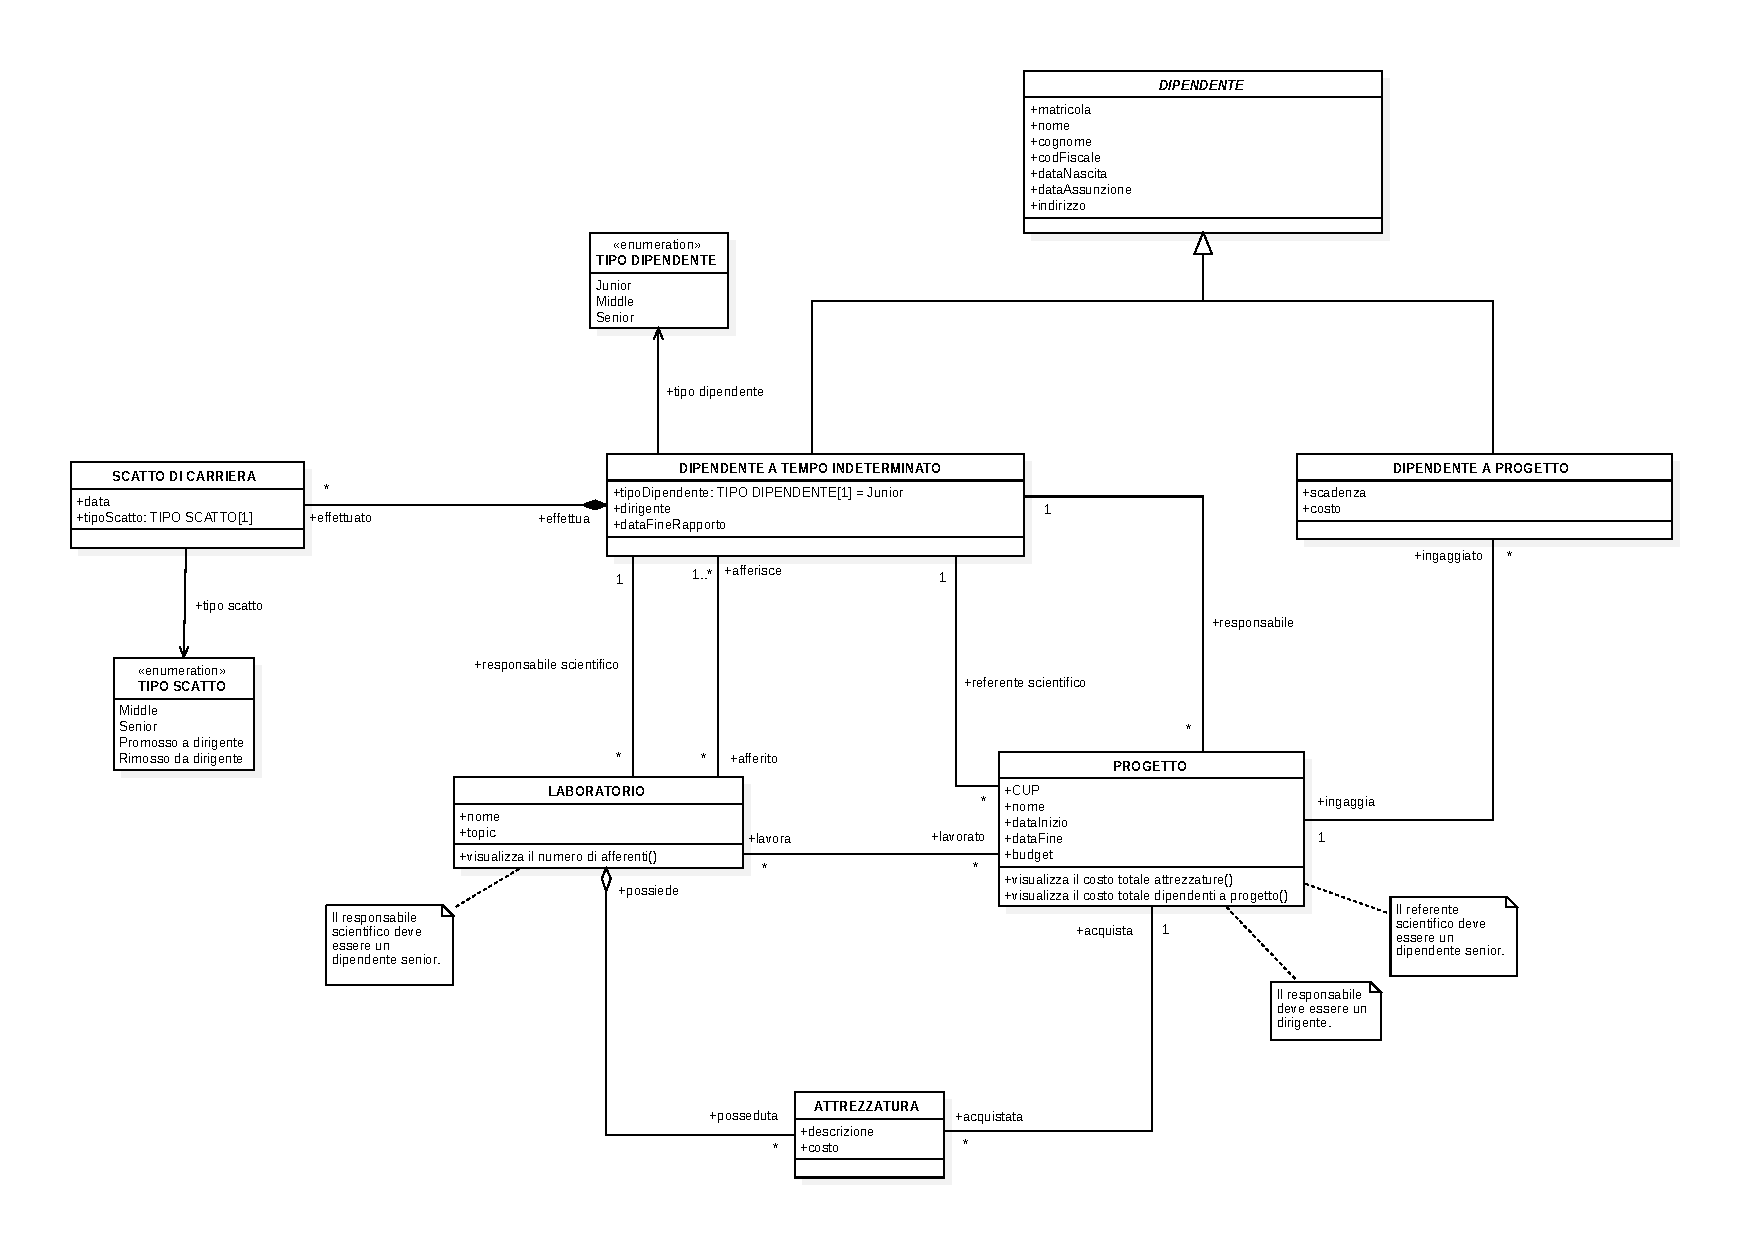
\includegraphics[width=\linewidth]{Immagini/Diagrammi/Class Diagram/Class diagram del dominio del problema.pdf}
            \caption{Class Diagram del dominio del problema}
            \label{fig:Class Diagram del dominio del problema}
        \end{figure}

    \section{Dizionario delle classi}
        \begin{tabular}{|C{3.5cm}|L{11.2cm}|}
            \hline
            \multicolumn{1}{|c|}{\textbf{Classe}} & \multicolumn{1}{c|}{\textbf{Descrizione}}\\  
            \hline
                DIPENDENTE &
                La classe "Dipendente" è una generalizzazione di "Dipendente a tempo indeterminato" e "Dipendente a progetto". Queste ultime due classi erediteranno gli attributi di "Dipendente": la matricola, il nome, il cognome, il codice fiscale, l'indirizzo di residenza, la data di nascita, la data di assunzione.\\
            \hline
                DIPENDENTE CON CONTRATTO A TEMPO INDETERMINATO &
                La classe "Dipendente a tempo indeterminato" rappresenta i dipendenti assunti con contratto a tempo indeterminato dall'azienda. Eredita da "Dipendente". Agli attributi di "Dipendente", aggiungiamo la data di fine rapporto (ovvero la data in cui eventualmente smette di prestare servizio nell'azienda), un attributo tipo che specifica l'anzianità del dipendente (ovvero se è un dipendente Junior, Middle o Senior) e un attributo che indica se il dipendente è attualmente un dirigente o meno.\\
            \hline
                SCATTO DI CARRIERA &
                La classe "Scatto di carriera" rappresenta gli scatti di carriera di un dipendente. In particolare lo scatto può essere di quattro tipi:
                \begin{enumerate}
                    \item Scatto da junior a middle, indicato con "Middle"
                    \item Scatto da middle a senior, indicato con "Senior"
                    \item Scatto da non dirigente a dirigente, che indichiamo con la denominazione "Promosso a dirigente", non vincolato all'anzianità
                    \item Scatto da dirigente a non dirigente, che indichiamo con la denominazione "Rimosso da dirigente", non vincolato all'anzianità.
                \end{enumerate}
                Oltre al tipo di scatto avremo anche la data in cui è avvenuto lo scatto per una determinata matricola.\\
            \hline
                LABORATORIO &
                La classe "Laboratorio" rappresenta i laboratori che si trovano attualmente all'interno dell'azienda. In particolare un laboratorio avrà un nome e un topic.\\
            \hline
                ATTREZZATURA &
                La classe "Attrezzatura" rappresenta le attrezzature acquistate tramite i fondi di progetti, che possono o meno trovarsi all'interno di un laboratorio. In particolare, un'attrezzatura è un oggetto che avrà un costo e una descrizione (che appunto descrive l'oggetto in questione).\\
            \hline
                PROGETTO &
                La classe "Progetto" rappresenta i progetti presi in carico dall'azienda. In particolare il progetto possiederà un CUP (Codice Unico Progetto), un nome, una data di inizio e di fine esecuzione del progetto e il budget totale (che rappresenta i fondi istanziati per quel progetto)\\
            \hline
                DIPENDENTE CON "CONTRATTO A PROGETTO" &
                La classe "Dipendente a progetto" rappresenta i dipendenti assunti per lavorare su un progetto tramite un contratto a tempo determinato. Eredita da "Dipendente". Agli attributi di "Dipendente", aggiungiamo una data di scadenza (ovvero la data in cui scade il contratto a tempo determinato) e un costo.\\
            \hline   
        \end{tabular}
        
    \section{Dizionario delle associazioni}
        \begin{tabular}{|C{3.5cm}|L{11.2cm}|}
            \hline
                \multicolumn{1}{|c|}{\textbf{Associazione}} &
                \multicolumn{1}{c|}{\textbf{Descrizione}}\\            
            \hline
                SCATTO DI CARRIERA ... DIPENDENTE A TEMPO INDETERMINATO &
                L'associazione tra "DIPENDENTE CON CONTRATTO A TEMPO INDETERMINATO" e "SCATTO DI CARRIERA" è un'associazione volta a identificare gli "SCATTI DI CARRIERA" del relativo dipendente. In particolare, un dipendente può avere diversi scatti di carriera, o nessuno. Viceversa, uno scatto è relativo ad un unico dipendente.\\
            \hline
                TIPO SCATTO ... SCATTO DI CARRIERA &
                L'associazione tra "SCATTO DI CARRIERA" e la classe enumerativa "TIPO SCATTO" specifica quali sono i possibili valori che può assumere l'attributo "Tipo" di "SCATTO DI CARRIERA". Da un "TIPO SCATTO" non è possibile risalire a tutti gli oggetti "SCATTO DI CARRIERA" che hanno quel "TIPO SCATTO" nell'attributo "Tipo". Ogni attributo "Tipo" dello scatto di carriera può assumere un solo valore tra quelli del "TIPO SCATTO".\\
            \hline
                TIPO DIPENDENTE ... DIPENDENTE CON CONTRATTO A TEMPO INDETERMINATO &
                L'associazione tra "DIPENDENTE CON CONTRATTO A TEMPO" e la classe enumerativa "TIPO DIPENDENTE" specifica quali sono i possibili valori che può assumere l'attributo "Tipo" di "DIPENDENTE CON CONTRATTO A TEMPO INDETERMINATO". Da un "TIPO DIPENDENTE" non è possibile risalire a tutti gli oggetti "DIPENDENTE CON CONTRATTO A TEMPO INDETERMINATO" che hanno quel "TIPO DIPENDENTE" nell'attributo "Tipo". Ogni attributo "Tipo" del dipendente può assumere un solo valore tra quelli del "TIPO DIPENDENTE".\\
            \hline
                DIPENDENTE CON CONTRATTO A TEMPO INDETERMINATO ... LABORATORIO &
                L'associazione "RESPONSABILE SCIENTIFICO" tra "DIPENDENTE CON CONTRATTO A TEMPO INDETERMINATO" e "LABORATORIO" specifica quali dipendenti sono responsabili scientifici di un laboratorio. In particolare, un dipendete potrebbe essere, o meno, responsabile scientifico di uno o più laboratori. Viceversa, un laboratorio avrà uno ed un solo responsabile scientifico.\\
            \hline
                DIPENDENTE CON CONTRATTO A TEMPO INDETERMINATO ... LABORATORIO &
                L'associazione "AFFERIRE" tra "DIPENDENTE CON CONTRATTO A TEMPO INDETERMINATO" e "LABORATORIO" indica quali sono i dipendenti che afferiscono attualmente ad un particolare laboratorio. In particolar modo, un dipendente può afferire a più laboratori, ma potrebbe anche non afferirne a nessuno. Viceversa, un laboratorio può avere più afferenti, oltre al responsabile scientifico.\\
            \hline
                DIPENDENTE CON CONTRATTO A TEMPO INDETERMINATO ... PROGETTO &
                L'associazione "REFERENTE SCIENTIFICO" tra "DIPENDENTE CON CONTRATTO A TEMPO INDETERMINATO" e "PROGETTO" denota quali dipendenti sono referenti scientifici di un progetto. In particolare, un dipendente potrebbe essere, o meno, referente scientifico di uno o più progetti. Al contrario, un progetto deve avere uno ed un solo referente scientifico.\\
            \hline
                DIPENDENTE CON CONTRATTO A TEMPO INDETERMINATO ... PROGETTO &
                L'associazione "RESPONSABILE" tra "DIPENDENTE CON CONTRATTO A TEMPO INDETERMINATO" e "PROGETTO" indica quali dipendenti sono responsabili di un progetto. In particolare, un dipendete potrebbe essere, o meno, responsabile di uno o più progetti, mentre un progetto avrà uno ed un solo responsabile.\\
            \hline
        \end{tabular}

        \begin{tabular}{|C{3.5cm}|L{11.2cm}|}
            \hline
                \multicolumn{1}{|c|}{\textbf{Associazione}} &
                \multicolumn{1}{c|}{\textbf{Descrizione}}\\
            \hline
                LABORATORIO ... PROGETTO &
                L'associazione tra "LABORATORIO" e "PROGETTO" fa corrispondere, ad ogni laboratorio, i progetti a cui ha lavorato. In particolare, un laboratorio può aver lavorato a più progetti, così come potrebbe non aver mai lavorato ad alcun progetto. Viceversa, un progetto presenta almeno un laboratorio che ha lavorato ad esso, fino a un massimo di tre.\\
            \hline
                LABORATORIO ... ATTREZZATURA &
                L'associazione tra "LABORATORIO" e "ATTREZZATURA" indica le attrezzature appartenenti ad un laboratorio. Un laboratorio potrebbe avere più attrezzature, così come potrebbe non averne nessuna. All'opposto, un'attrezzatura appartiene, o meno, ad un laboratorio.\\
            \hline
                ATTREZZATURA ... PROGETTO &
                L'associazione tra "ATTREZZATURA" e "PROGETTO" fornisce informazioni circa le attrezzature acquistate tramite i fondi di un progetto. Sarà possibile acquistare più attrezzature, o nessuna, per un progetto. Invece, tutte le attrezzature, se acquistate, devono essere acquistate tramite i fondi di uno ed un solo progetto.\\
            \hline
                PROGETTO ... DIPENDENTE CON CONTRATTO A PROGETTO &
                L'associazione tra "PROGETTO" e "DIPENDENTE CON CONTRATTO A PROGETTO" indica quali sono i dipendenti ingaggiati utilizzando il budget di un progetto. Infatti, sarà possibile ingaggiare più dipendenti con contratto a progetto, o nessuno. Viceversa, un dipendente con contratto a progetto, se presente, è stato assunto mediante i fondi di uno ed un solo progetto.\\
            \hline
        \end{tabular}
    \chapter{Diagramma di dettaglio delle classi nel dominio della soluzione}
    \section{Class Diagram del dominio della soluzione}
        Di seguito è riportato il Class Diagram del dominio della soluzione.\\
        In particolare, il tipo di visibilità è espressa da questa tabella:
        \begin{figure}[htbp!]
                \centering
                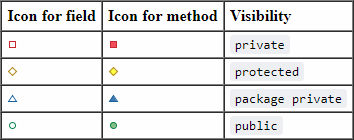
\includegraphics[width=0.25\linewidth]{Immagini/Legend visibility.png}
            \caption{Legenda della visibilità}
            \label{fig:Legenda della visibilità}
        \end{figure}\\
        Inoltre, i costruttori della classe sono i metodi contrassegnati da \textless{}\textless{}Create\textgreater{}\textgreater{}.

        %Class Diagram costruito con PlantUML
        \begin{figure}[htbp!]
            \centering
                \vspace{2\baselineskip}
                \includegraphics[width=\linewidth]{Immagini/Diagrammi/Class Diagram/Class Diagram del dominio della soluzione.pdf}
            \caption{Class Diagram del dominio della soluzione}
            \label{fig:Class Diagram del dominio della soluzione}
        \end{figure}
    \chapter{Sequence Diagram}
    \section{Sequence Diagram leggiLavorare}
        %Class Diagram costruito con StarUML
        \begin{figure}[htbp!]
            \centering
                \vspace{2\baselineskip}
                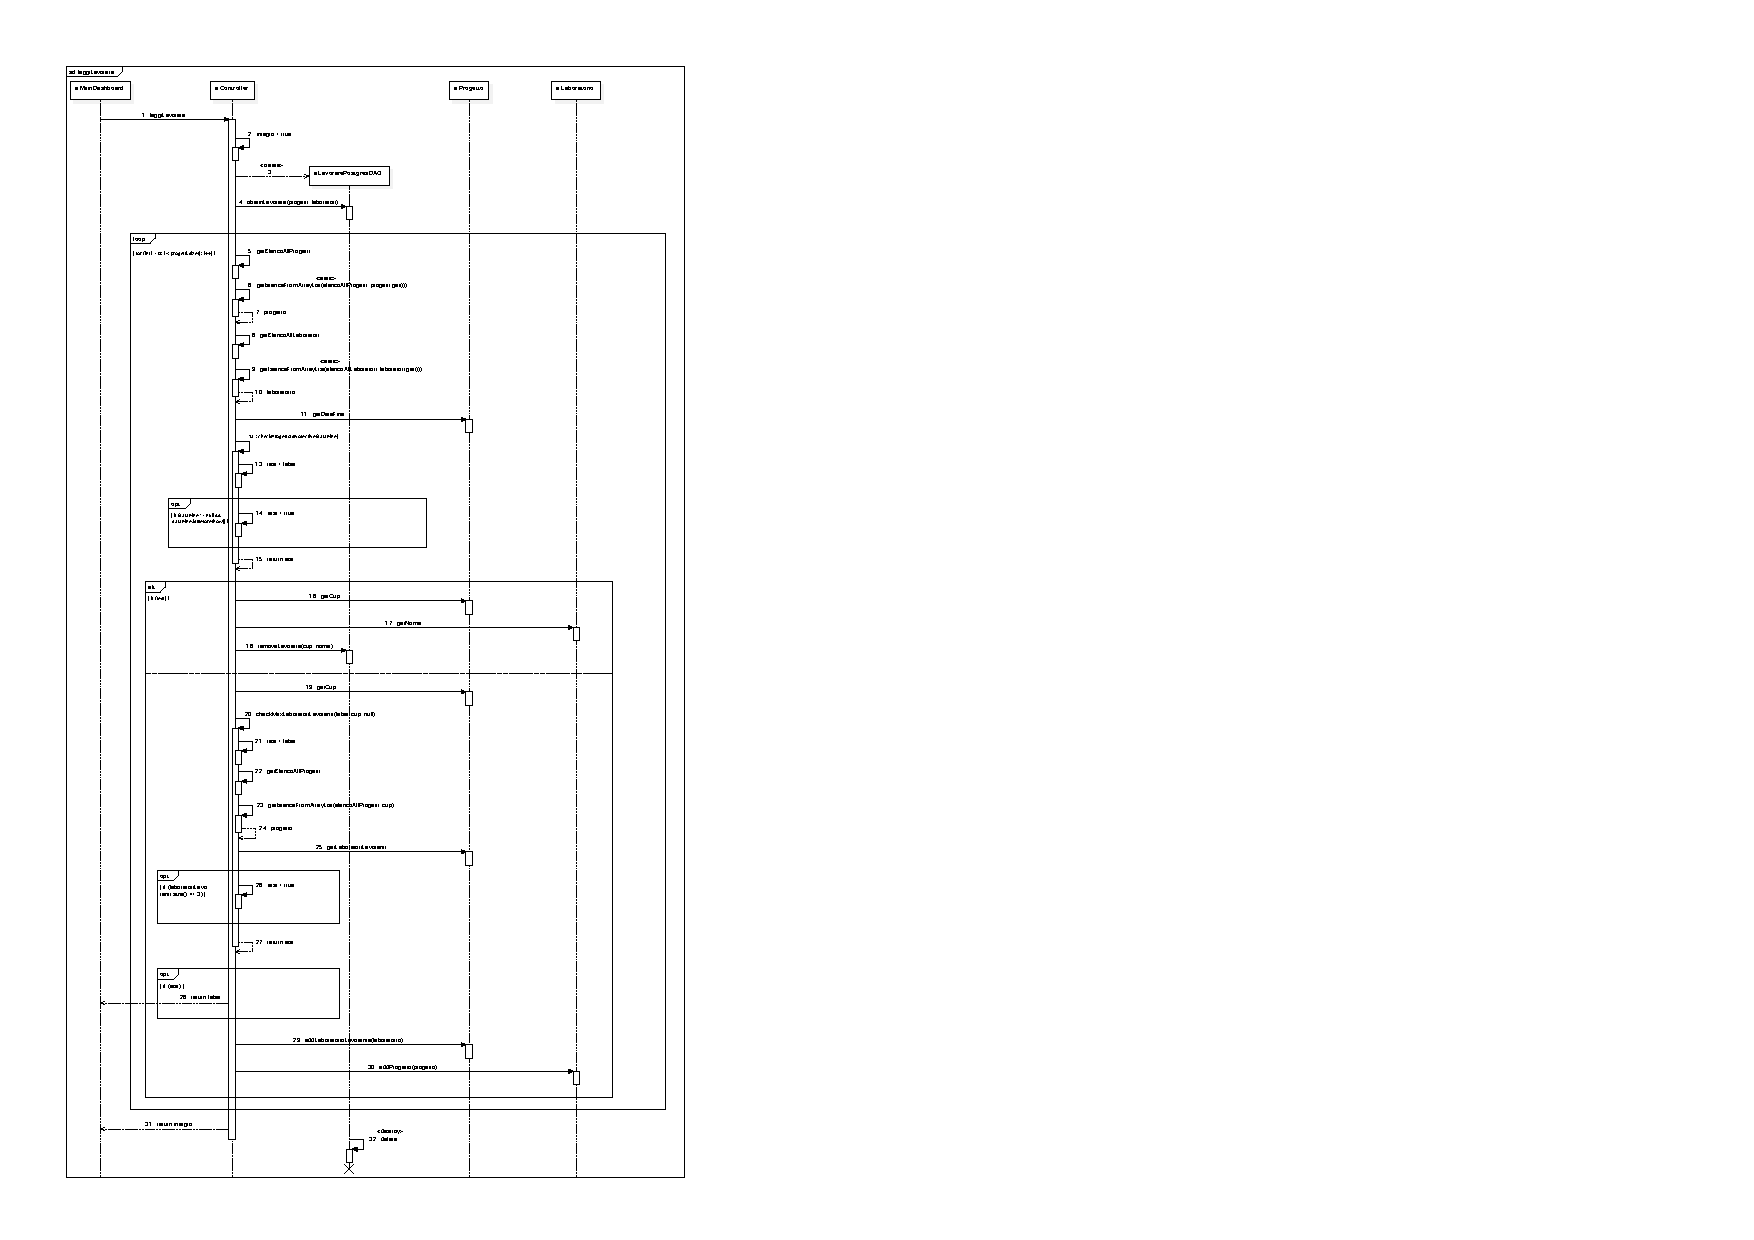
\includegraphics[width=1.3\linewidth]{Immagini/Diagrammi/Sequence Diagram/Sequence Diagram leggiLavorare.pdf}
            \caption{Sequence Diagram leggiLavorare}
            \label{fig:Sequence Diagram leggiLavorare}
        \end{figure}

    \newpage

    \section{Sequence Diagram leggiLaboratori}
        %Class Diagram costruito con StarUML
        \begin{figure}[htbp!]
            \centering
                \vspace{2\baselineskip}
                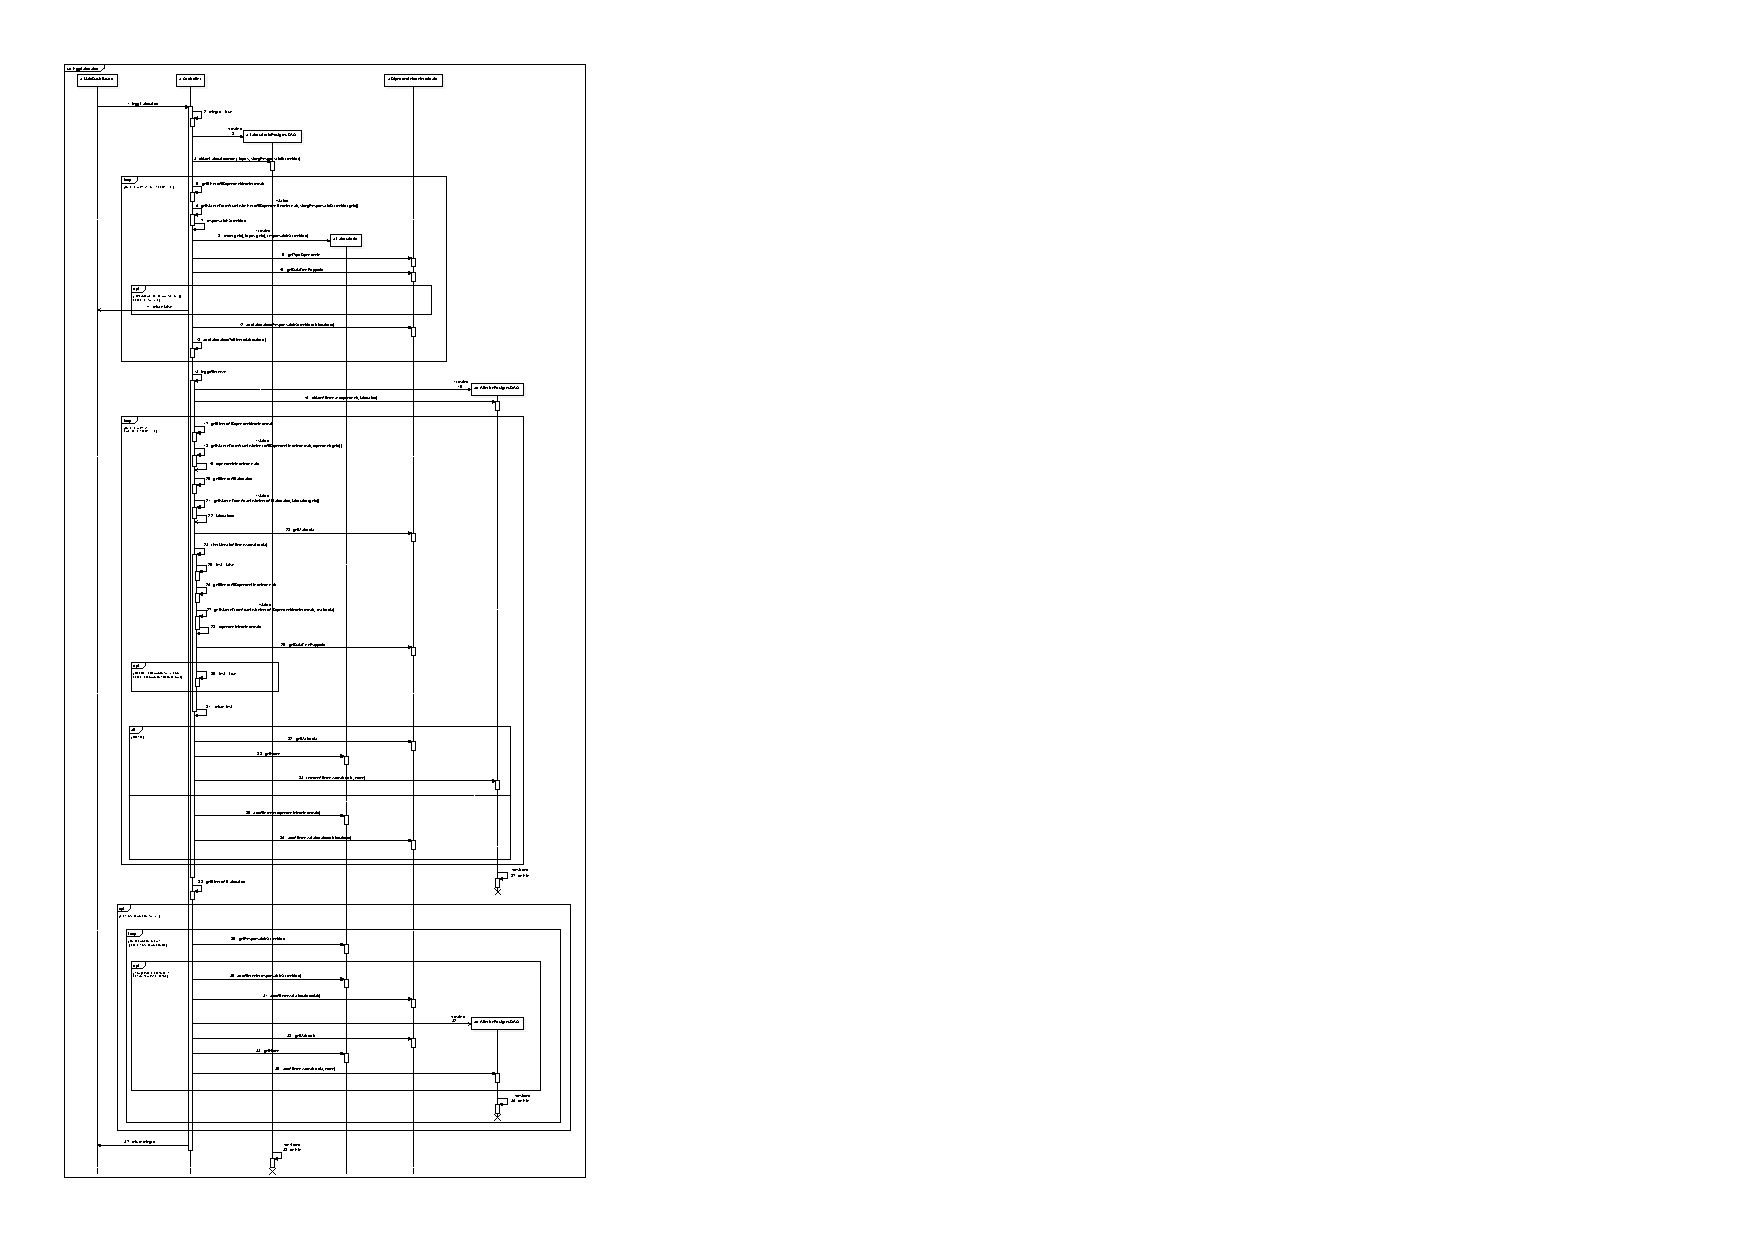
\includegraphics[width=1.7\linewidth]{Immagini/Diagrammi/Sequence Diagram/Sequence Diagram leggiLaboratori.pdf}
            \caption{Sequence Diagram leggiLaboratori}
            \label{fig:Sequence Diagram leggiLaboratori}
        \end{figure}
    \chapter{Descrizione dell'applicativo}
    \section{Descrizione generale}
        L'applicativo denominato "SIRIUS" (Sistema Informativo Relazionale Integrato per l'Umane Risorse) permette la gestione di un database per la gestione di personale, laboratori e progetti all'interno dell'azienda. Attraverso diverse sezioni è possibile mostrare i dati relativi a quella sezione nel database. E' anche possibile aggiungere, modificare ed eliminare dati dal database.

    \section{Frames Home}
        Nella finestra "Home" l'utente può decidere a quale area accedere da cui poi effettuare le operazioni abilitate per quell'area.
        \begin{figure}[htbp!]
            \centering
                \vspace{2\baselineskip}
                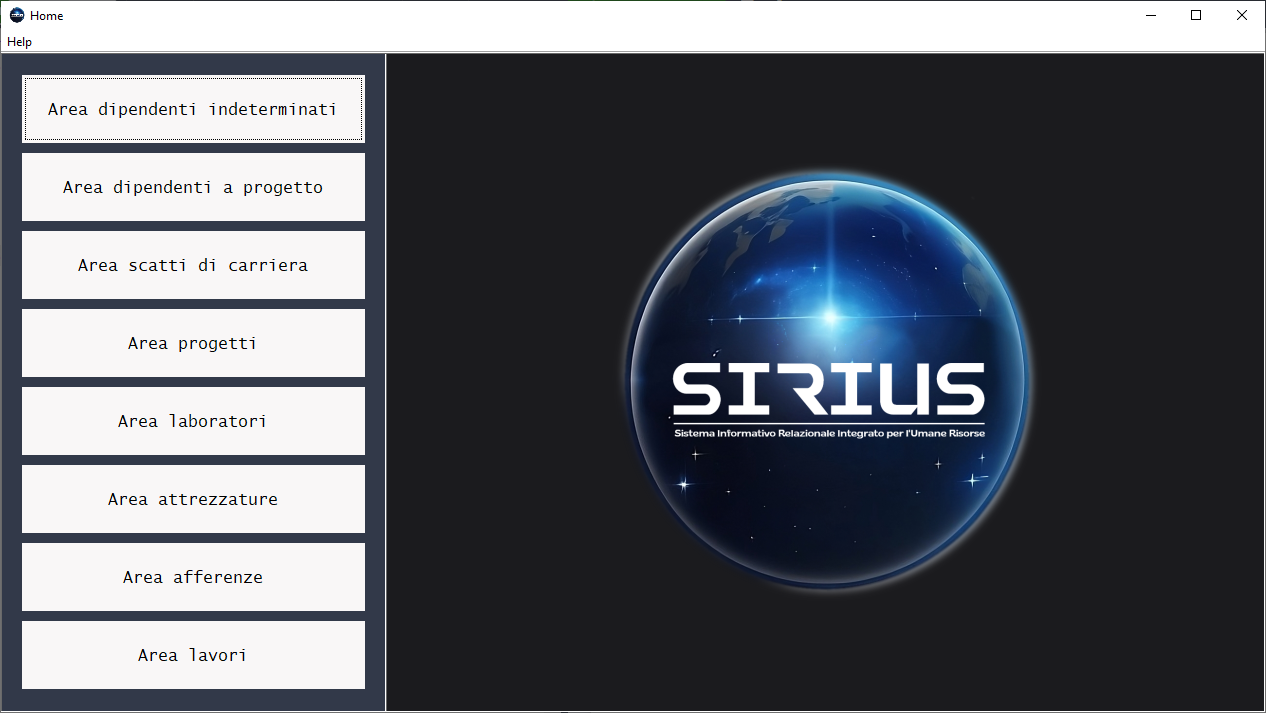
\includegraphics[width=0.9\linewidth]{Immagini/Frames/Frame Home.png}
            \caption{Frame Home}
            \label{fig:Frame Home}
        \end{figure}

    \newpage

    \section{Frames Dipendenti indeterminati}
        \subsection {Finestra "Area dipendenti indeterminati"}
            Nella finestra "Area dipendenti indeterminati" l'utente avrà a disposizione una tabella con tutti i dati nel database relativi ai dipendenti assunti a tempo indeterminato. Ogni colonna può essere ordinata in senso crescente o decrescente.\\
            Da qui, attraverso i bottoni in basso, si potrà decidere se tornare alla schermata home (indietro), aggiungere un nuovo dipendente a tempo indeterminato (aggiungi) o selezionare un dipendente e modificarne i dati (modifica). Cliccando su "aggiungi" o "modifica" si aprirà la finestra "aggiungi/modifica Dipendenti indeterminati". Dato che si intende tenere traccia di tutti i dipendenti a tempo indeterminato, non è possibile eliminarne alcuno dall'applicativo.\\
            In alto è inoltre presente una barra di ricerca. I valori inseriti al suo interno saranno cercati tra tutti i campi della tabella.
            \begin{figure}[htbp!]
                \centering
                    \vspace{2\baselineskip}
                    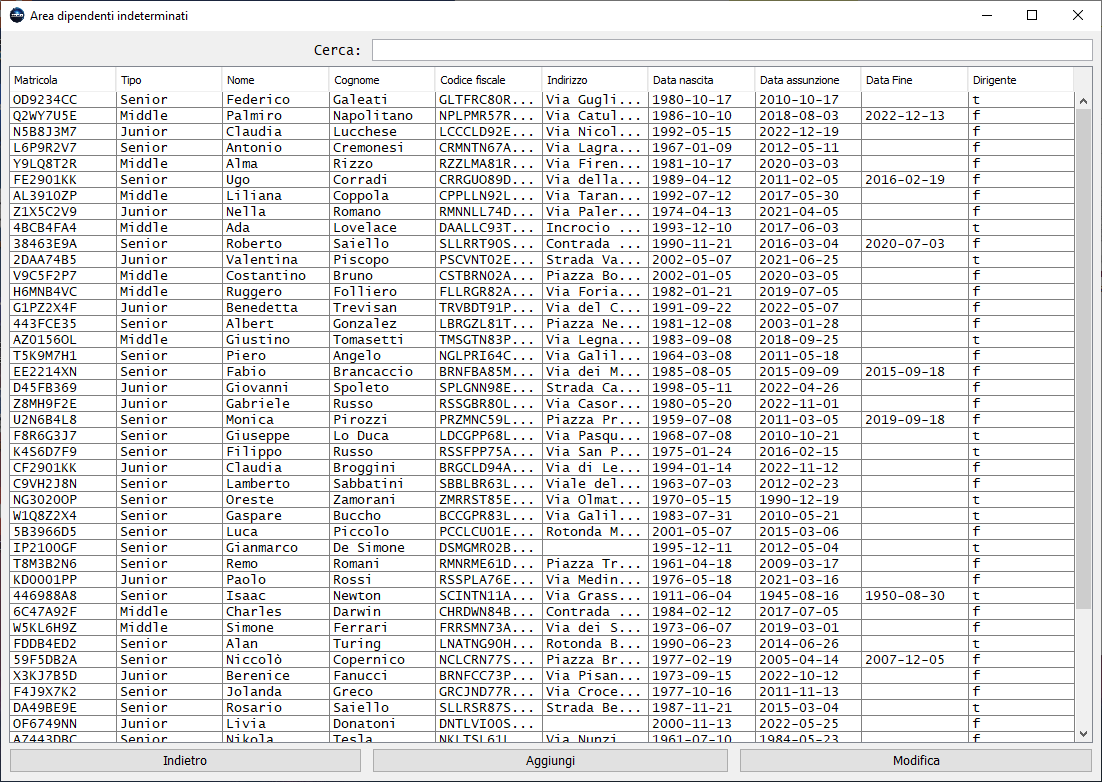
\includegraphics[width=0.9\linewidth]{Immagini/Frames/Frame Area/Frame Area dipendenti indeterminati.png}
                \caption{Frame Area dipendenti indeterminati}
                \label{fig:Frame Area dipendenti indeterminati}
            \end{figure}

    \newpage

        \subsection {Finestra "aggiungi/modifica Dipendenti indeterminati"}
            Nella finestra "aggiungi/modifica Dipendenti indeterminati" l'utente potrà inserire i valori negli appositi campi per aggiungere un dipendente al database. In particolare, potrà inserire nome, cognome, codice fiscale, matricola, tipo dipendente (e spuntare la relativa checkbox se si intende aggiungere un dirigente), indirizzo (il campo sarà abilitato spuntando la relativa checkbox), data di nascita, data di assunzione (spuntando la relativa checkbox il campo verrà automaticamente compilato con la data odierna) e la data di fine rapporto (spuntando la prima checkbox si rende disponibile il campo, mentre con la seconda checkbox si compila automaticamente con la data odierna).\\
            Con i bottoni in basso si può annullare o confermare l'aggiunta.\\
            Se, invece, nella finestra "Area dipendente indeterminato" si è cliccati su "modifica", i campi verranno precompilati con quelli del dipendente selezionato. Dopodichè si potrà procedere con la modifica.
            \begin{figure}[htbp!]
                \centering
                    \vspace{2\baselineskip}
                    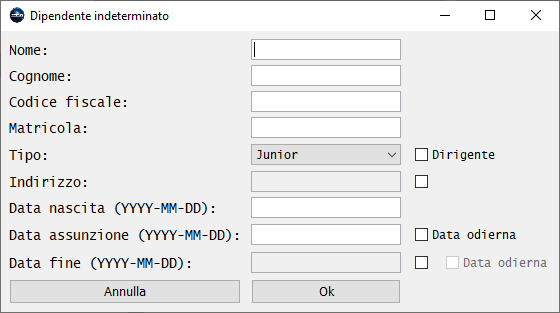
\includegraphics[width=0.6\linewidth]{Immagini/Frames/Frame aggiungi-modifica/Frame Dipendente indeterminato aggiungi-modifica.png}
                \caption{Frame Dipendente indeterminato aggiungi-modifica}
                \label{fig:Frame Dipendente indeterminato aggiungi-modifica}
            \end{figure}

    \newpage

    \section{Frames Dipendenti a progetto}
        \subsection {Finestra "Area dipendenti progetto"}
            Nella finestra "Area dipendenti progetto" l'utente avrà a disposizione una tabella con tutti i dati nel database relativi ai dipendenti assunti con contratto a progetto. Ogni colonna può essere ordinata in senso crescente o decrescente.\\
            Da qui, attraverso i bottoni in basso, si potrà decidere se tornare alla schermata home (indietro), aggiungere un nuovo dipendente a tempo a progetto (aggiungi) o selezionare un dipendente e modificarne i dati (modifica). Cliccando su "aggiungi" o "modifica" si aprirà la finestra "aggiungi/modifica Dipendenti progetto". Dato che si intende tenere traccia di tutti i dipendenti con contratto a progetto, non è possibile eliminarne alcuno dall'applicativo.\\
            In alto è inoltre presente una barra di ricerca. I valori inseriti al suo interno saranno cercati tra tutti i campi della tabella.
            \begin{figure}[htbp!]
                \centering
                    \vspace{2\baselineskip}
                    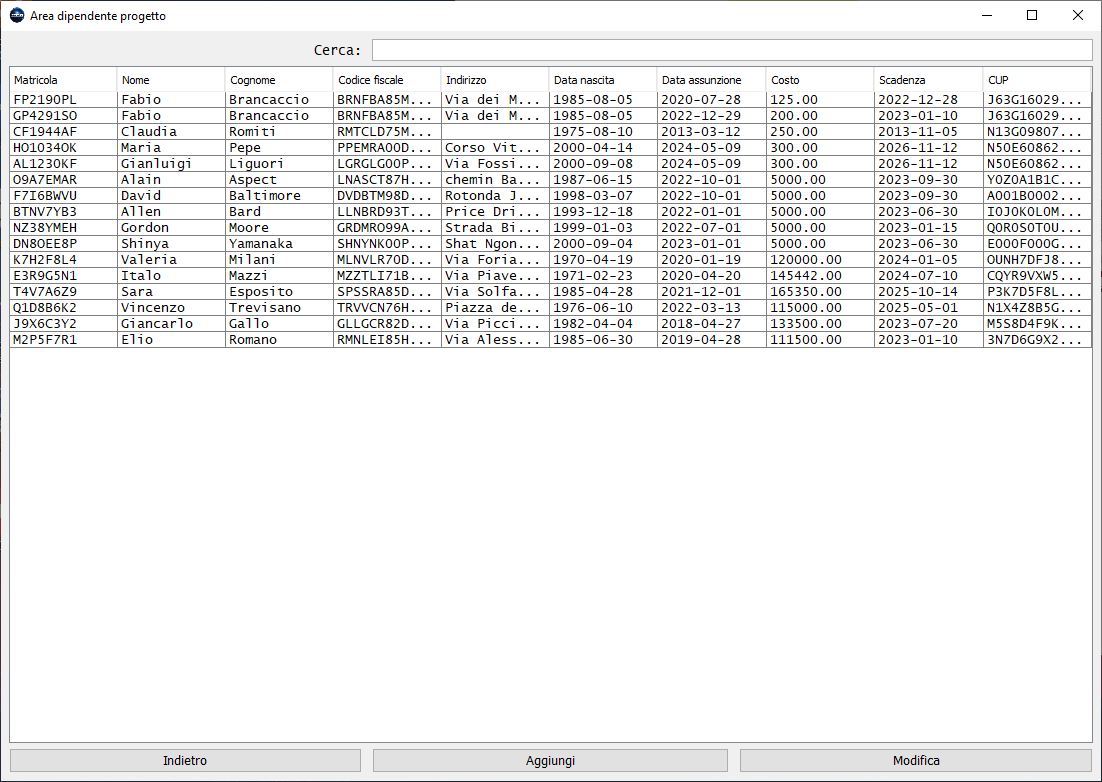
\includegraphics[width=0.9\linewidth]{Immagini/Frames/Frame Area/Frame Area dipendente progetto.png}
                \caption{Frame Area dipendenti progetto}
                \label{fig:Frame Area dipendenti progetto}
            \end{figure}

    \newpage

        \subsection {Finestra "aggiungi/modifica Dipendenti progetto"}
            Nella finestra "aggiungi/modifica Dipendenti progetto" l'utente potrà inserire i valori negli appositi campi per aggiungere un dipendente al database. In particolare, potrà inserire nome, cognome, codice fiscale, matricola, indirizzo (il campo sarà abilitato spuntando la relativa checkbox), data di nascita, data di assunzione (spuntando la relativa checkbox il campo verrà automaticamente compilato con la data odierna), la data di scadenza del contratto (spuntando la checkbox si compila automaticamente con la data odierna), il costo del contratto a progetto e quale progetto ha ingaggiato il dipendente che stiamo inserendo.\\
            Con i bottoni in basso si può annullare o confermare l'aggiunta.\\
            Se, invece, nella finestra "Area dipendente progetto" si è cliccati su "modifica", i campi verranno precompilati con quelli del dipendente selezionato. Dopodichè si potrà procedere con la modifica.
            \begin{figure}[htbp!]
                \centering
                    \vspace{2\baselineskip}
                    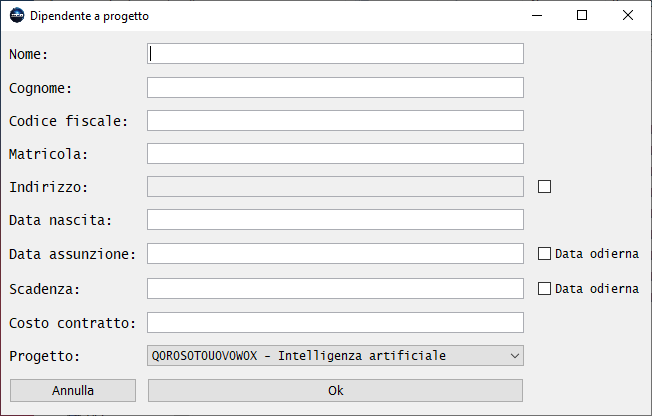
\includegraphics[width=0.6\linewidth]{Immagini/Frames/Frame aggiungi-modifica/Frame Dipendente a progetto aggiungi-modifica.png}
                \caption{Frame Dipendente a progetto aggiungi-modifica}
                \label{fig:Frame Dipendente a progetto aggiungi-modifica}
            \end{figure}

    \newpage

    \section{Frames Scatti di carriera}
        \subsection {Finestra "Area scatti di carriera"}
            Nella finestra "Area scatti di carriera" l'utente avrà a disposizione una tabella con tutti i dati nel database relativi agli scatti di carriera. Ogni colonna può essere ordinata in senso crescente o decrescente.\\
            Da qui, attraverso i bottoni in basso, si potrà decidere se tornare alla schermata home (indietro), aggiungere un nuovo scatti di carriera (aggiungi) o selezionare uno scatti di carriera di tipo dirigenziale e modificarne i dati (modifica). Cliccando su "aggiungi" o "modifica" si aprirà la finestra "aggiungi/modifica Dipendenti progetto". Dato che si intende tenere traccia di tutti gli scatti di carriera, non è possibile eliminarne alcuno tramite app. Inoltre, gli scatti di carriera di tipo "Middle" e "Senior" sono automaticamente gestiti dall'applicativo.\\
            In alto è inoltre presente una barra di ricerca. I valori inseriti al suo interno saranno cercati tra tutti i campi della tabella.
            \begin{figure}[htbp!]
                \centering
                    \vspace{2\baselineskip}
                    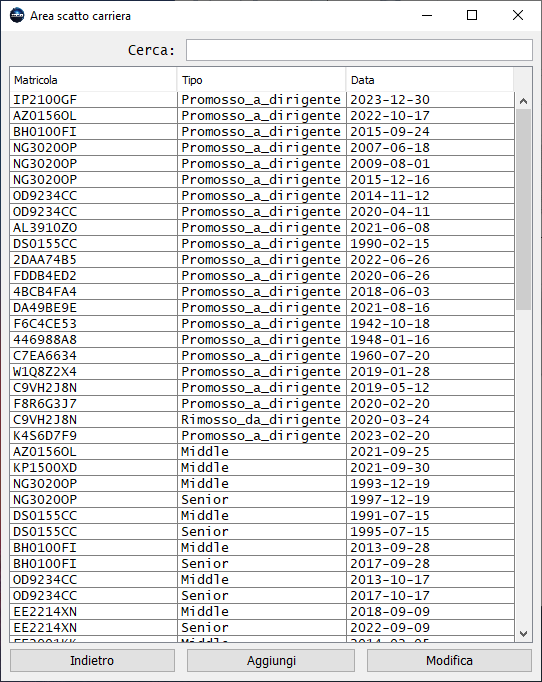
\includegraphics[width=0.6\linewidth]{Immagini/Frames/Frame Area/Frame Area scatto carriera.png}
                \caption{Frame Area scatto carriera}
                \label{fig:Frame Area scatto carriera}
            \end{figure}

    \newpage

        \subsection {Finestra "aggiungi/modifica Scatto carriera"}
            Nella finestra "aggiungi/modifica Scatto carriera" l'utente potrà inserire i valori negli appositi campi per aggiungere uno scatto di carriera al database. In particolare, potrà inserire il dipendente che effettua lo scatto, la data in cui viene effettuato (spuntando la relativa checkbox il campo verrà automaticamente compilato con la data odierna) e il tipo di scatto (gli scatti di tipo "Middle" e "Senior" sono automaticamente gestiti dall'applicativo). Per confermare il tipo di scatto è necessario cliccare su "Seleziona".\\
            Con i bottoni in basso si può annullare o confermare l'aggiunta.\\
            Se, invece, nella finestra "Area scatto carriera" si è cliccati su "modifica", i campi verranno precompilati con quelli dello scatto di carriera selezionato. Dopodichè si potrà procedere con la modifica.
            \begin{figure}[htbp!]
                \centering
                    \vspace{2\baselineskip}
                    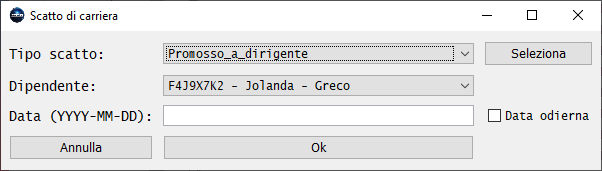
\includegraphics[width=0.7\linewidth]{Immagini/Frames/Frame aggiungi-modifica/Frame Scatto di carriera aggiungi-modifica.png}
                \caption{Frame Scatto carriera aggiungi-modifica}
                \label{fig:Frame Scatto carriera aggiungi-modifica}
            \end{figure}

    \newpage

    \section{Frames Progetto}
        \subsection {Finestra "Area progetto"}
            Nella finestra "Area progetto" l'utente avrà a disposizione una tabella con tutti i dati nel database relativi ai progetti. Ogni colonna può essere ordinata in senso crescente o decrescente.\\
            Da qui, attraverso i bottoni in basso, si potrà decidere se tornare alla schermata home (indietro), aggiungere un nuovo progetto (aggiungi) o selezionare un progetto e modificarne i dati (modifica). Cliccando su "aggiungi" o "modifica" si aprirà la finestra "aggiungi/modifica Progetto". Dato che si intende tenere traccia di tutti i progetti, non è possibile eliminarne alcuno tramite app.\\
            In alto è inoltre presente una barra di ricerca. I valori inseriti al suo interno saranno cercati tra tutti i campi della tabella.
            \begin{figure}[htbp!]
                \centering
                    \vspace{2\baselineskip}
                    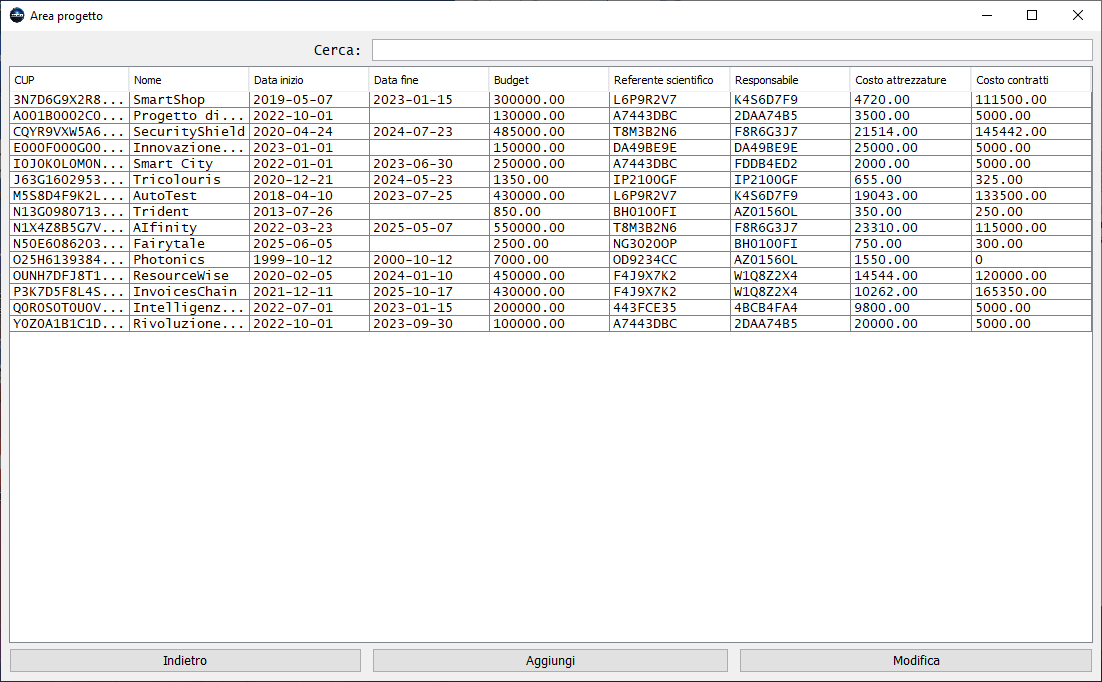
\includegraphics[width=0.9\linewidth]{Immagini/Frames/Frame Area/Frame Area progetto.png}
                \caption{Frame Area progetto}
                \label{fig:Frame Area progetto}
            \end{figure}

    \newpage

        \subsection {Finestra "aggiungi/modifica Progetto"}
            Nella finestra "aggiungi/modifica Progetto" l'utente potrà inserire i valori negli appositi campi per aggiungere un progetto al database. In particolare, potrà inserire il nome, il CUP, il budget istanziato per il progetto, la data di inizio progetto, la data di fine progetto (Si può rendere disponibile il campo spuntando la prima checkbox, confermare la data inserita cliccando su "Seleziona" e spuntare la seconda checkbox per precompilare il campo con la data odierna), il referente scientifico e il responsabile.\\
            Con i bottoni in basso si può annullare o confermare l'aggiunta.\\
            Se, invece, nella finestra "Area progetto" si è cliccati su "modifica", i campi verranno precompilati con quelli del progetto selezionato. Dopodichè si potrà procedere con la modifica.
            \begin{figure}[htbp!]
                \centering
                    \vspace{2\baselineskip}
                    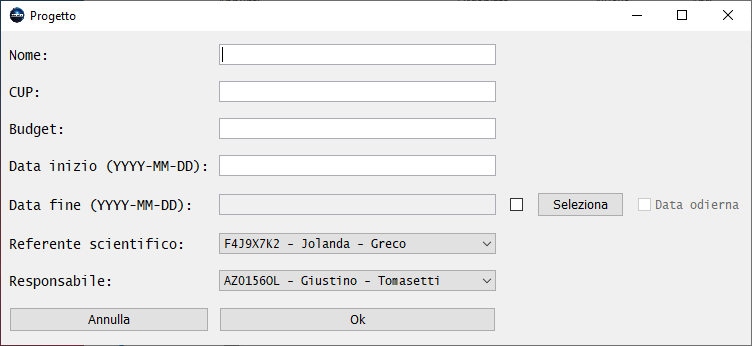
\includegraphics[width=0.7\linewidth]{Immagini/Frames/Frame aggiungi-modifica/Frame Progetto aggiungi-modifica.png}
                \caption{Frame Progetto aggiungi-modifica}
                \label{fig:Frame Progetto aggiungi-modifica}
            \end{figure}

    \newpage

    \section{Frames Laboratorio}
        \subsection {Finestra "Area laboratorio"}
            Nella finestra "Area laboratorio" l'utente avrà a disposizione una tabella con tutti i dati nel database relativi ai laboratori. Ogni colonna può essere ordinata in senso crescente o decrescente.\\
            Da qui, attraverso i bottoni in basso, si potrà decidere se tornare alla schermata home (indietro), aggiungere un nuovo laboratorio (aggiungi), selezionare un laboratorio e modificarne i dati (modifica) o eliminare il laboratorio selezionato. Cliccando su "aggiungi" o "modifica" si aprirà la finestra "aggiungi/modifica Laboratorio".\\
            In alto è inoltre presente una barra di ricerca. I valori inseriti al suo interno saranno cercati tra tutti i campi della tabella.
            \begin{figure}[htbp!]
                \centering
                    \vspace{2\baselineskip}
                    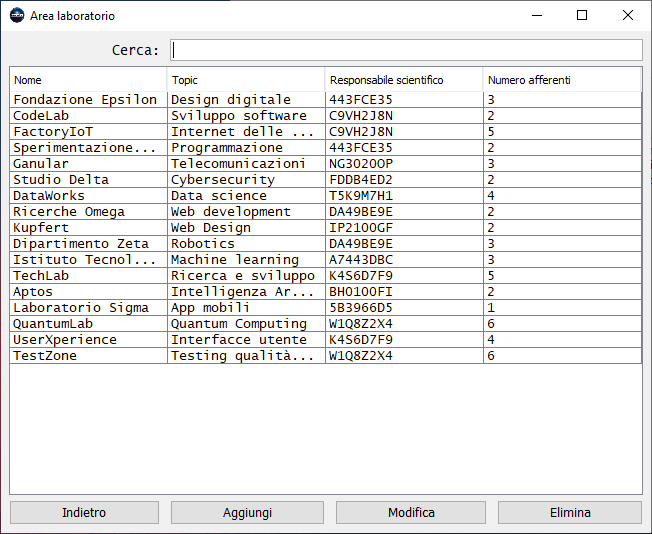
\includegraphics[width=0.9\linewidth]{Immagini/Frames/Frame Area/Frame Area laboratorio.png}
                \caption{Frame Area laboratorio}
                \label{fig:Frame Area laboratorio}
            \end{figure}

    \newpage

        \subsection {Finestra "aggiungi/modifica Laboratorio"}
            Nella finestra "aggiungi/modifica Laboratorio" l'utente potrà inserire i valori negli appositi campi per aggiungere un laboratorio al database. In particolare, potrà inserire il nome, il topic e il responsabile scientifico.\\
            Con i bottoni in basso si può annullare o confermare l'aggiunta.\\
            Se, invece, nella finestra "Area laboratorio" si è cliccati su "modifica", i campi verranno precompilati con quelli del laboratorio selezionato. Dopodichè si potrà procedere con la modifica.
            \begin{figure}[htbp!]
                \centering
                    \vspace{2\baselineskip}
                    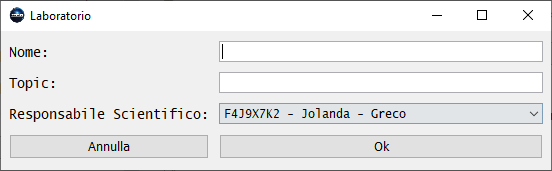
\includegraphics[width=0.7\linewidth]{Immagini/Frames/Frame aggiungi-modifica/Frame Laboratorio aggiungi-modifica.png}
                \caption{Frame Laboratorio aggiungi-modifica}
                \label{fig:Frame Laboratorio aggiungi-modifica}
            \end{figure}

    \newpage

    \section{Frames Attrezzatura}
        \subsection {Finestra "Area attrezzatura"}
            Nella finestra "Area attrezzatura" l'utente avrà a disposizione una tabella con tutti i dati nel database relativi alle attrezzature. Ogni colonna può essere ordinata in senso crescente o decrescente.\\
            Da qui, attraverso i bottoni in basso, si potrà decidere se tornare alla schermata home (indietro), aggiungere una nuova attrezzatura (aggiungi) o selezionare un'attrezzatura e modificarne i dati (modifica). Cliccando su "aggiungi" o "modifica" si aprirà la finestra "aggiungi/modifica Attrezzatura". Dato che si intende tenere traccia di tutte le attrezzature, non è possibile eliminarne alcuna tramite app.\\
            In alto è inoltre presente una barra di ricerca. I valori inseriti al suo interno saranno cercati tra tutti i campi della tabella.
            \begin{figure}[htbp!]
                \centering
                    \vspace{2\baselineskip}
                    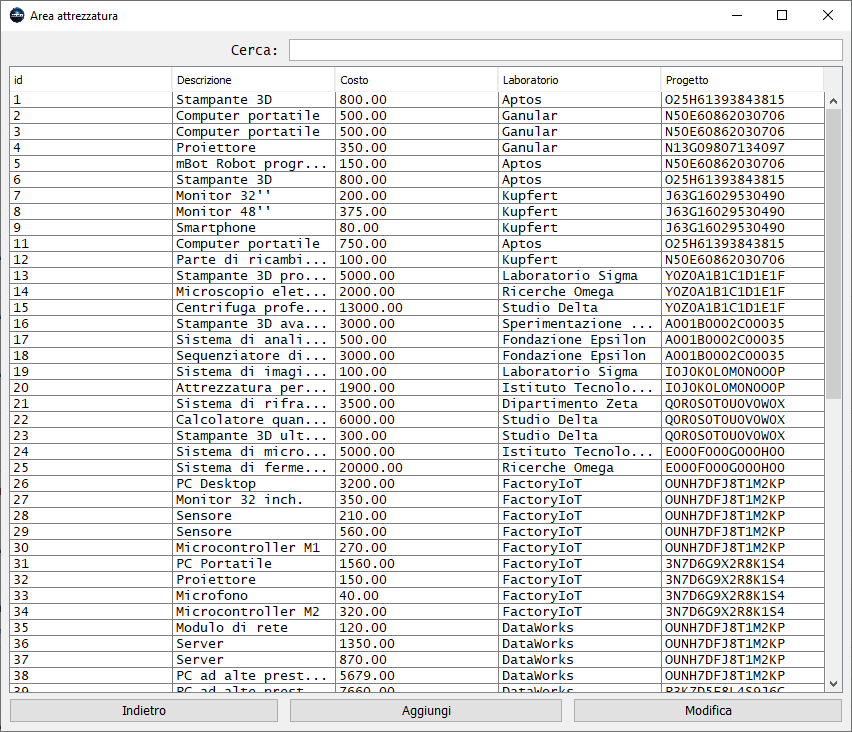
\includegraphics[width=0.9\linewidth]{Immagini/Frames/Frame Area/Frame Area attrezzatura.png}
                \caption{Frame Area attrezzatura}
                \label{fig:Frame Area attrezzatura}
            \end{figure}

    \newpage

        \subsection {Finestra "aggiungi/modifica Attrezzatura"}
            Nella finestra "aggiungi/modifica Attrezzatura" l'utente potrà inserire i valori negli appositi campi per aggiungere un'attrezzatura al database. In particolare, potrà inserire la descrizione, il costo, il progetto che ha acquistato l'attrezzatura (una volta scelto, è necessario confermare cliccando su "Seleziona") e il laboratorio a è stata assegnata, se esiste (il campo può essere abilitato tramite l'apposita checkbox)\\
            Con i bottoni in basso si può annullare o confermare l'aggiunta.\\
            Se, invece, nella finestra "Area attrezzatura" si è cliccati su "modifica", i campi verranno precompilati con quelli del laboratorio selezionato. Dopodichè si potrà procedere con la modifica.
            \begin{figure}[htbp!]
                \centering
                    \vspace{2\baselineskip}
                    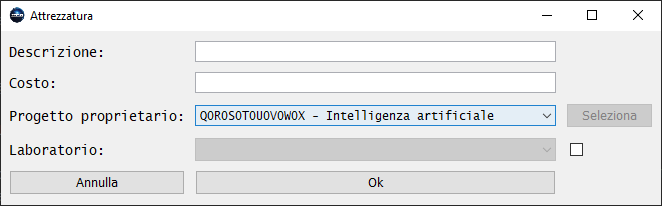
\includegraphics[width=0.7\linewidth]{Immagini/Frames/Frame aggiungi-modifica/Frame Attrezzatura aggiungi-modifica.png}
                \caption{Frame Attrezzatura aggiungi-modifica}
                \label{fig:Frame Attrezzatura aggiungi-modifica}
            \end{figure}

    \newpage

    \section{Frames Afferenze}
        \subsection {Finestra "Area afferenze"}
            Nella finestra "Area afferenze" l'utente avrà a disposizione una tabella con tutti i dati nel database relativi alle afferenze ai laboratori. Ogni colonna può essere ordinata in senso crescente o decrescente.\\
            Da qui, attraverso i bottoni in basso, si potrà decidere se tornare alla schermata home (indietro), aggiungere una nuova afferenza (aggiungi), selezionare un'afferenza e modificarne i dati (modifica) o eliminare l'afferenza selezionata. Cliccando su "aggiungi" o "modifica" si aprirà la finestra "aggiungi/modifica Afferenza".\\
            In alto è inoltre presente una barra di ricerca. I valori inseriti al suo interno saranno cercati tra tutti i campi della tabella.
            \begin{figure}[htbp!]
                \centering
                    \vspace{2\baselineskip}
                    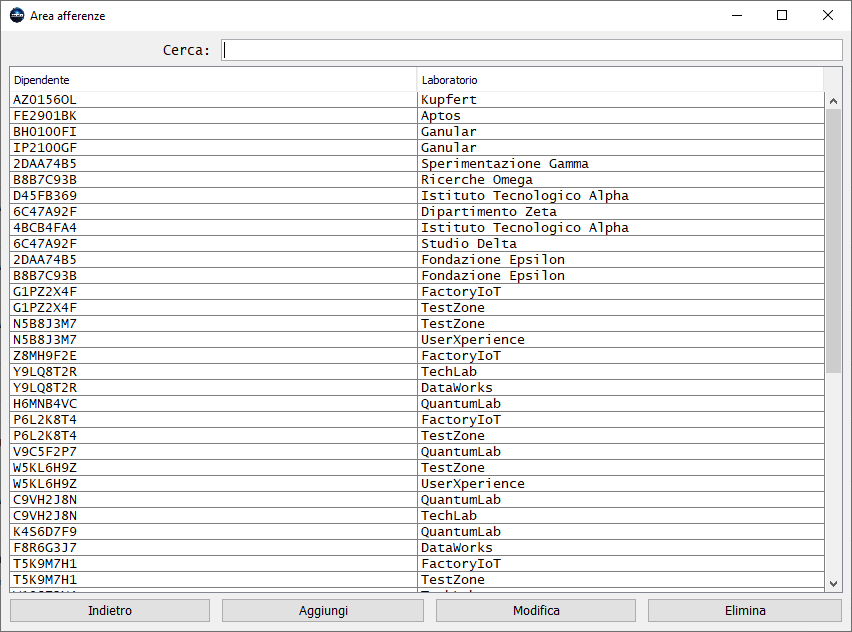
\includegraphics[width=0.9\linewidth]{Immagini/Frames/Frame Area/Frame Area afferenze.png}
                \caption{Frame Area afferenze}
                \label{fig:Frame Area afferenze}
            \end{figure}

    \newpage

        \subsection {Finestra "aggiungi/modifica Afferenza"}
            Nella finestra "aggiungi/modifica Afferenza" l'utente potrà inserire i valori negli appositi campi per aggiungere un'afferenza al database. In particolare, potrà inserire il dipendente e il laboratorio a cui afferisce.\\
            Con i bottoni in basso si può annullare o confermare l'aggiunta.\\
            Se, invece, nella finestra "Area afferenza" si è cliccati su "modifica", i campi verranno precompilati con quelli dell'afferenza selezionata. Dopodichè si potrà procedere con la modifica.
            \begin{figure}[htbp!]
                \centering
                    \vspace{2\baselineskip}
                    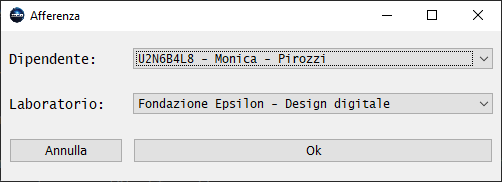
\includegraphics[width=0.7\linewidth]{Immagini/Frames/Frame aggiungi-modifica/Frame Afferenza aggiungi-modifica.png}
                \caption{Frame Afferenza aggiungi-modifica}
                \label{fig:Frame Afferenza aggiungi-modifica}
            \end{figure}

    \newpage

    \section{Frames Lavorare}
        \subsection {Finestra "Area lavorare"}
            Nella finestra "Area lavorare" l'utente avrà a disposizione una tabella con tutti i dati nel database relativi alle associazioni di "lavorare" tra laboratori e progetti. Ogni colonna può essere ordinata in senso crescente o decrescente.\\
            Da qui, attraverso i bottoni in basso, si potrà decidere se tornare alla schermata home (indietro), aggiungere un nuovo lavoro (aggiungi), selezionare un lavoro e modificarne i dati (modifica) o eliminare il lavoro selezionato. Cliccando su "aggiungi" o "modifica" si aprirà la finestra "aggiungi/modifica Lavorare".\\
            In alto è inoltre presente una barra di ricerca. I valori inseriti al suo interno saranno cercati tra tutti i campi della tabella.
            \begin{figure}[htbp!]
                \centering
                    \vspace{2\baselineskip}
                    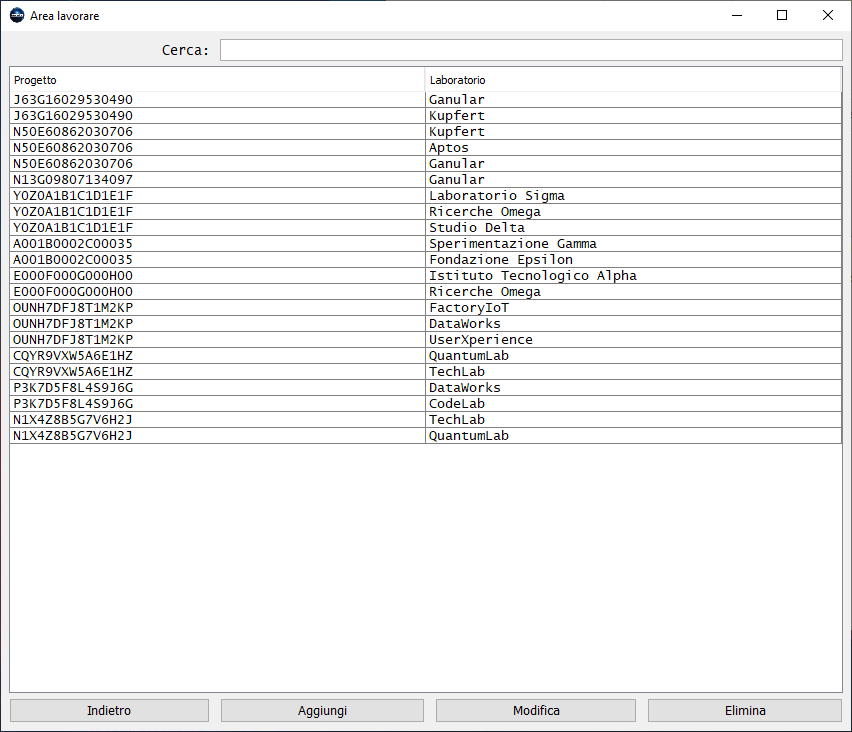
\includegraphics[width=0.9\linewidth]{Immagini/Frames/Frame Area/Frame Area lavorare.png}
                \caption{Frame Area lavorare}
                \label{fig:Frame Area lavorare}
            \end{figure}

    \newpage

        \subsection {Finestra "aggiungi/modifica Lavorare"}
            Nella finestra "aggiungi/modifica Lavori" l'utente potrà inserire i valori negli appositi campi per aggiungere un'associazione di lavoro tra laboratorio e progetto al database. In particolare, potrà inserire il progetto e il laboratorio che ci lavora.\\
            Con i bottoni in basso si può annullare o confermare l'aggiunta.\\
            Se, invece, nella finestra "Area lavorare" si è cliccati su "modifica", i campi verranno precompilati con quelli del laboratorio selezionato. Dopodichè si potrà procedere con la modifica.
            \begin{figure}[htbp!]
                \centering
                    \vspace{2\baselineskip}
                    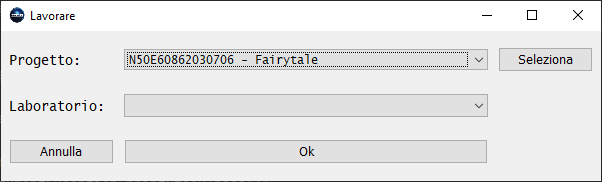
\includegraphics[width=0.7\linewidth]{Immagini/Frames/Frame aggiungi-modifica/Frame Lavorare aggiungi-modifica.png}
                \caption{Frame Lavorare aggiungi-modifica}
                \label{fig:Frame Lavorare aggiungi-modifica}
            \end{figure}
    
\end{document}